% Options for packages loaded elsewhere
\PassOptionsToPackage{unicode}{hyperref}
\PassOptionsToPackage{hyphens}{url}
%
\documentclass[
]{article}
\title{The Personality Structures of the 50 States}
\author{Anisha Babu, Diana DeWald, Ian Shryock, Dillon Welindt, Futing Zou}
\date{}

\usepackage{amsmath,amssymb}
\usepackage{lmodern}
\usepackage{iftex}
\ifPDFTeX
  \usepackage[T1]{fontenc}
  \usepackage[utf8]{inputenc}
  \usepackage{textcomp} % provide euro and other symbols
\else % if luatex or xetex
  \usepackage{unicode-math}
  \defaultfontfeatures{Scale=MatchLowercase}
  \defaultfontfeatures[\rmfamily]{Ligatures=TeX,Scale=1}
\fi
% Use upquote if available, for straight quotes in verbatim environments
\IfFileExists{upquote.sty}{\usepackage{upquote}}{}
\IfFileExists{microtype.sty}{% use microtype if available
  \usepackage[]{microtype}
  \UseMicrotypeSet[protrusion]{basicmath} % disable protrusion for tt fonts
}{}
\makeatletter
\@ifundefined{KOMAClassName}{% if non-KOMA class
  \IfFileExists{parskip.sty}{%
    \usepackage{parskip}
  }{% else
    \setlength{\parindent}{0pt}
    \setlength{\parskip}{6pt plus 2pt minus 1pt}}
}{% if KOMA class
  \KOMAoptions{parskip=half}}
\makeatother
\usepackage{xcolor}
\IfFileExists{xurl.sty}{\usepackage{xurl}}{} % add URL line breaks if available
\IfFileExists{bookmark.sty}{\usepackage{bookmark}}{\usepackage{hyperref}}
\hypersetup{
  pdftitle={The Personality Structures of the 50 States},
  pdfauthor={Anisha Babu, Diana DeWald, Ian Shryock, Dillon Welindt, Futing Zou},
  hidelinks,
  pdfcreator={LaTeX via pandoc}}
\urlstyle{same} % disable monospaced font for URLs
\usepackage[margin=1in]{geometry}
\usepackage{color}
\usepackage{fancyvrb}
\newcommand{\VerbBar}{|}
\newcommand{\VERB}{\Verb[commandchars=\\\{\}]}
\DefineVerbatimEnvironment{Highlighting}{Verbatim}{commandchars=\\\{\}}
% Add ',fontsize=\small' for more characters per line
\usepackage{framed}
\definecolor{shadecolor}{RGB}{248,248,248}
\newenvironment{Shaded}{\begin{snugshade}}{\end{snugshade}}
\newcommand{\AlertTok}[1]{\textcolor[rgb]{0.94,0.16,0.16}{#1}}
\newcommand{\AnnotationTok}[1]{\textcolor[rgb]{0.56,0.35,0.01}{\textbf{\textit{#1}}}}
\newcommand{\AttributeTok}[1]{\textcolor[rgb]{0.77,0.63,0.00}{#1}}
\newcommand{\BaseNTok}[1]{\textcolor[rgb]{0.00,0.00,0.81}{#1}}
\newcommand{\BuiltInTok}[1]{#1}
\newcommand{\CharTok}[1]{\textcolor[rgb]{0.31,0.60,0.02}{#1}}
\newcommand{\CommentTok}[1]{\textcolor[rgb]{0.56,0.35,0.01}{\textit{#1}}}
\newcommand{\CommentVarTok}[1]{\textcolor[rgb]{0.56,0.35,0.01}{\textbf{\textit{#1}}}}
\newcommand{\ConstantTok}[1]{\textcolor[rgb]{0.00,0.00,0.00}{#1}}
\newcommand{\ControlFlowTok}[1]{\textcolor[rgb]{0.13,0.29,0.53}{\textbf{#1}}}
\newcommand{\DataTypeTok}[1]{\textcolor[rgb]{0.13,0.29,0.53}{#1}}
\newcommand{\DecValTok}[1]{\textcolor[rgb]{0.00,0.00,0.81}{#1}}
\newcommand{\DocumentationTok}[1]{\textcolor[rgb]{0.56,0.35,0.01}{\textbf{\textit{#1}}}}
\newcommand{\ErrorTok}[1]{\textcolor[rgb]{0.64,0.00,0.00}{\textbf{#1}}}
\newcommand{\ExtensionTok}[1]{#1}
\newcommand{\FloatTok}[1]{\textcolor[rgb]{0.00,0.00,0.81}{#1}}
\newcommand{\FunctionTok}[1]{\textcolor[rgb]{0.00,0.00,0.00}{#1}}
\newcommand{\ImportTok}[1]{#1}
\newcommand{\InformationTok}[1]{\textcolor[rgb]{0.56,0.35,0.01}{\textbf{\textit{#1}}}}
\newcommand{\KeywordTok}[1]{\textcolor[rgb]{0.13,0.29,0.53}{\textbf{#1}}}
\newcommand{\NormalTok}[1]{#1}
\newcommand{\OperatorTok}[1]{\textcolor[rgb]{0.81,0.36,0.00}{\textbf{#1}}}
\newcommand{\OtherTok}[1]{\textcolor[rgb]{0.56,0.35,0.01}{#1}}
\newcommand{\PreprocessorTok}[1]{\textcolor[rgb]{0.56,0.35,0.01}{\textit{#1}}}
\newcommand{\RegionMarkerTok}[1]{#1}
\newcommand{\SpecialCharTok}[1]{\textcolor[rgb]{0.00,0.00,0.00}{#1}}
\newcommand{\SpecialStringTok}[1]{\textcolor[rgb]{0.31,0.60,0.02}{#1}}
\newcommand{\StringTok}[1]{\textcolor[rgb]{0.31,0.60,0.02}{#1}}
\newcommand{\VariableTok}[1]{\textcolor[rgb]{0.00,0.00,0.00}{#1}}
\newcommand{\VerbatimStringTok}[1]{\textcolor[rgb]{0.31,0.60,0.02}{#1}}
\newcommand{\WarningTok}[1]{\textcolor[rgb]{0.56,0.35,0.01}{\textbf{\textit{#1}}}}
\usepackage{longtable,booktabs,array}
\usepackage{calc} % for calculating minipage widths
% Correct order of tables after \paragraph or \subparagraph
\usepackage{etoolbox}
\makeatletter
\patchcmd\longtable{\par}{\if@noskipsec\mbox{}\fi\par}{}{}
\makeatother
% Allow footnotes in longtable head/foot
\IfFileExists{footnotehyper.sty}{\usepackage{footnotehyper}}{\usepackage{footnote}}
\makesavenoteenv{longtable}
\usepackage{graphicx}
\makeatletter
\def\maxwidth{\ifdim\Gin@nat@width>\linewidth\linewidth\else\Gin@nat@width\fi}
\def\maxheight{\ifdim\Gin@nat@height>\textheight\textheight\else\Gin@nat@height\fi}
\makeatother
% Scale images if necessary, so that they will not overflow the page
% margins by default, and it is still possible to overwrite the defaults
% using explicit options in \includegraphics[width, height, ...]{}
\setkeys{Gin}{width=\maxwidth,height=\maxheight,keepaspectratio}
% Set default figure placement to htbp
\makeatletter
\def\fps@figure{htbp}
\makeatother
\setlength{\emergencystretch}{3em} % prevent overfull lines
\providecommand{\tightlist}{%
  \setlength{\itemsep}{0pt}\setlength{\parskip}{0pt}}
\setcounter{secnumdepth}{5}
\usepackage{tocbibind}
\usepackage{booktabs}
\usepackage{longtable}
\usepackage{array}
\usepackage{multirow}
\usepackage{wrapfig}
\usepackage{float}
\usepackage{colortbl}
\usepackage{pdflscape}
\usepackage{tabu}
\usepackage{threeparttable}
\usepackage{threeparttablex}
\usepackage[normalem]{ulem}
\usepackage{makecell}
\usepackage{xcolor}
\ifLuaTeX
  \usepackage{selnolig}  % disable illegal ligatures
\fi

\begin{document}
\maketitle

{
\setcounter{tocdepth}{2}
\tableofcontents
}
\renewcommand{\thetable}{\arabic{table}} 
\renewcommand{\thefigure}{\arabic{figure}}

\definecolor{fancyTextColor}{HTML}{4284f5}
\definecolor{hightlightColor}{HTML}{FFFF66}

\newpage

\listoftables

\newpage

\begin{Shaded}
\begin{Highlighting}[]
\NormalTok{SAPA }\OtherTok{\textless{}{-}}\NormalTok{ SAPA }\SpecialCharTok{\%\textgreater{}\%}
  \CommentTok{\# filter in US}
  \FunctionTok{filter}\NormalTok{(country }\SpecialCharTok{==} \StringTok{"USA"}\NormalTok{) }\SpecialCharTok{\%\textgreater{}\%}
  \CommentTok{\# filter 50 states}
  \FunctionTok{filter}\NormalTok{(}\SpecialCharTok{!}\NormalTok{state }\SpecialCharTok{\%in\%} \FunctionTok{c}\NormalTok{(}\StringTok{\textquotesingle{}District of Columbia\textquotesingle{}}\NormalTok{, }
                       \StringTok{\textquotesingle{}Guam\textquotesingle{}}\NormalTok{, }
                       \StringTok{\textquotesingle{}Palau\textquotesingle{}}\NormalTok{,}
                       \StringTok{\textquotesingle{}Puerto Rico\textquotesingle{}}\NormalTok{, }
                       \StringTok{\textquotesingle{}Virgin Islands\textquotesingle{}}\NormalTok{,}
                       \StringTok{\textquotesingle{}Northern Mariana Islands\textquotesingle{}}\NormalTok{, }
                       \StringTok{\textquotesingle{}American Samoa\textquotesingle{}}\NormalTok{, }
                       \StringTok{\textquotesingle{}Marshall Islands\textquotesingle{}}\NormalTok{, }
                       \ConstantTok{NA}\NormalTok{)) }

\CommentTok{\# filter out rows with all NA}
\NormalTok{SAPA }\OtherTok{\textless{}{-}}\NormalTok{ SAPA[}\FunctionTok{rowSums}\NormalTok{(}\FunctionTok{is.na}\NormalTok{(SAPA)) }\SpecialCharTok{\textless{}} \DecValTok{99}\NormalTok{, ]}

\CommentTok{\# in list form select only used Q\textquotesingle{}s}
\NormalTok{usedQ }\OtherTok{\textless{}{-}} \FunctionTok{colnames}\NormalTok{(SAPA[}\DecValTok{8}\SpecialCharTok{:}\DecValTok{106}\NormalTok{])}

\NormalTok{IPIPkeys }\OtherTok{\textless{}{-}} \FunctionTok{map}\NormalTok{(IPIPkeysList, }\ControlFlowTok{function}\NormalTok{(x) \{}
\NormalTok{    x[}\FunctionTok{match}\NormalTok{(usedQ, x)]}
    \FunctionTok{na.omit}\NormalTok{(x)}
\NormalTok{\})}

\CommentTok{\# select only IPIP 100}
\NormalTok{IPIPkeys }\OtherTok{\textless{}{-}}\NormalTok{ IPIPkeys[}\DecValTok{1}\SpecialCharTok{:}\DecValTok{4}\NormalTok{]}
\end{Highlighting}
\end{Shaded}

\begin{verbatim}
## $gender
## 
## Female   Male 
##  56901  24465 
## 
## $age
## 
##   14   15   16   17   18   19   20   21   22   23   24   25   26   27   28   29 
##  767 1113 3129 6462 7707 6709 5896 4885 3621 2999 2569 2300 2193 2085 1887 1649 
##   30   31   32   33   34   35   36   37   38   39   40   41   42   43   44   45 
## 1590 1453 1345 1230 1212 1240 1152 1159 1069  958 1010  840  866  847  815  791 
##   46   47   48   49   50   51   52   53   54   55   56   57   58   59   60   61 
##  688  691  681  626  665  542  537  500  433  389  309  301  246  217  212  126 
##   62   63   64   65   66   67   68   69   70   71   72   73   74   75   76   77 
##  132   88   68   82   50   47   29   27   27   22   21    6   12    7    5    4 
##   78   79   80   81   82   83   84   85   86   87   88   89   90 
##    5    3    4    1    1    2    1    3    2    2    1    2    1 
## 
## $state
## 
##        Alabama         Alaska        Arizona       Arkansas     California 
##            643            555            866            577           9709 
##       Colorado    Connecticut       Delaware        Florida        Georgia 
##           1097            986            592           2936           2414 
##         Hawaii          Idaho       Illinois        Indiana           Iowa 
##            292            340           5520           1707            982 
##         Kansas       Kentucky      Louisiana          Maine       Maryland 
##            808            820           2030            356           1772 
##  Massachusetts       Michigan      Minnesota    Mississippi       Missouri 
##           1935           2549           2104            604           1611 
##        Montana       Nebraska         Nevada  New Hampshire     New Jersey 
##            243            580            274            389           2495 
##     New Mexico       New York North Carolina   North Dakota           Ohio 
##           1199           4942           1454            190           3600 
##       Oklahoma         Oregon   Pennsylvania   Rhode Island South Carolina 
##            771           1203           4758            422           1010 
##   South Dakota      Tennessee          Texas           Utah        Vermont 
##            172           1133           4662            487            161 
##       Virginia     Washington  West Virginia      Wisconsin        Wyoming 
##           2787           1742            384           2377            126 
## 
## $race
## 
## African American          Chinese Indian/Pakistani         Japanese 
##             6108             1129              469              257 
##           Korean           Latino          Mexican  Native American 
##              500             2079             2166              728 
##            Other      Other Asian Pacific Islander        Philipino 
##             3067              566              305              615 
##     Puerto Rican  White/Caucasian 
##              512            62859 
## 
## $education
## 
##                College graduate     Currently attending college 
##                           12381                           32469 
## Graduate or professional degree            High school graduate 
##                           10338                            6145 
##              Less than 12 years   Some college did not graduate 
##                           11759                            8274
\end{verbatim}

\begin{Shaded}
\begin{Highlighting}[]
\CommentTok{\# score items}
\NormalTok{scores }\OtherTok{\textless{}{-}}\NormalTok{ psych}\SpecialCharTok{::}\FunctionTok{scoreItems}\NormalTok{(}\AttributeTok{keys =}\NormalTok{ IPIPkeys, }\AttributeTok{items =}\NormalTok{ SAPA, }\AttributeTok{min =} \DecValTok{1}\NormalTok{, }\AttributeTok{max =} \DecValTok{6}\NormalTok{, }
                            \AttributeTok{totals =} \ConstantTok{FALSE}\NormalTok{, }\AttributeTok{impute =} \StringTok{\textquotesingle{}none\textquotesingle{}}\NormalTok{)}\SpecialCharTok{$}\NormalTok{scores}
\end{Highlighting}
\end{Shaded}

\begin{Shaded}
\begin{Highlighting}[]
\CommentTok{\# demographic table}
\NormalTok{demog\_tab }\OtherTok{\textless{}{-}} \FunctionTok{summary}\NormalTok{(}\FunctionTok{tableby}\NormalTok{(}\SpecialCharTok{\textasciitilde{}}\NormalTok{ age }\SpecialCharTok{+}\NormalTok{ gender }\SpecialCharTok{+}\NormalTok{ race }\SpecialCharTok{+}\NormalTok{ education, }
                             \AttributeTok{data =}\NormalTok{ SAPA, }\AttributeTok{test =} \ConstantTok{FALSE}\NormalTok{),  }
                     \AttributeTok{title =} \StringTok{"Full Sample Demographics"}\NormalTok{)}

\NormalTok{demog\_tab}
\end{Highlighting}
\end{Shaded}

\begin{longtable}[]{@{}lc@{}}
\caption{(\#tab:\#3 descriptives statistics)Full Sample Demographics}\tabularnewline
\toprule
& Overall (N=81366) \\
\midrule
\endfirsthead
\toprule
& Overall (N=81366) \\
\midrule
\endhead
\textbf{age} & \\
~~~Mean (SD) & 27.177 (11.343) \\
~~~Range & 14.000 - 90.000 \\
\textbf{gender} & \\
~~~Female & 56901 (69.9\%) \\
~~~Male & 24465 (30.1\%) \\
\textbf{race} & \\
~~~N-Miss & 6 \\
~~~African American & 6108 (7.5\%) \\
~~~Chinese & 1129 (1.4\%) \\
~~~Indian/Pakistani & 469 (0.6\%) \\
~~~Japanese & 257 (0.3\%) \\
~~~Korean & 500 (0.6\%) \\
~~~Latino & 2079 (2.6\%) \\
~~~Mexican & 2166 (2.7\%) \\
~~~Native American & 728 (0.9\%) \\
~~~Other & 3067 (3.8\%) \\
~~~Other Asian & 566 (0.7\%) \\
~~~Pacific Islander & 305 (0.4\%) \\
~~~Philipino & 615 (0.8\%) \\
~~~Puerto Rican & 512 (0.6\%) \\
~~~White/Caucasian & 62859 (77.3\%) \\
\textbf{education} & \\
~~~College graduate & 12381 (15.2\%) \\
~~~Currently attending college & 32469 (39.9\%) \\
~~~Graduate or professional degree & 10338 (12.7\%) \\
~~~High school graduate & 6145 (7.6\%) \\
~~~Less than 12 years & 11759 (14.5\%) \\
~~~Some college did not graduate & 8274 (10.2\%) \\
\bottomrule
\end{longtable}

\begin{Shaded}
\begin{Highlighting}[]
\CommentTok{\# PEER REVIEW: To get a more elegant table, perhaps you can create your own function that gives you the sample size and percent of sample size by different characteristic and then use map to create a data frame with the categories of choice. I wrote a function below to get you started.}

\NormalTok{sample }\OtherTok{\textless{}{-}} \ControlFlowTok{function}\NormalTok{(df,x) \{}
\NormalTok{  df }\SpecialCharTok{\%\textgreater{}\%}
  \FunctionTok{group\_by}\NormalTok{(\{\{x\}\}) }\SpecialCharTok{\%\textgreater{}\%}
  \FunctionTok{summarize}\NormalTok{(}\AttributeTok{group\_sample =} \FunctionTok{n}\NormalTok{()) }\SpecialCharTok{\%\textgreater{}\%}
  \FunctionTok{ungroup}\NormalTok{() }\SpecialCharTok{\%\textgreater{}\%}
  \FunctionTok{rename}\NormalTok{(}\AttributeTok{group =}\NormalTok{ \{\{x\}\}) }\SpecialCharTok{\%\textgreater{}\%}
  \FunctionTok{mutate}\NormalTok{(}\AttributeTok{total\_sample =} \FunctionTok{sum}\NormalTok{(group\_sample),}
         \AttributeTok{percent\_sample =}\NormalTok{ group\_sample}\SpecialCharTok{/}\NormalTok{total\_sample) }\SpecialCharTok{\%\textgreater{}\%}
  \FunctionTok{select}\NormalTok{(group,group\_sample, percent\_sample)}
\NormalTok{\}}

\FunctionTok{sample}\NormalTok{(SAPA,race)}
\end{Highlighting}
\end{Shaded}

\hypertarget{a-tibble-15-x-3}{%
\section{A tibble: 15 x 3}\label{a-tibble-15-x-3}}

group group\_sample percent\_sample
1 African American 6108 0.0751\\
2 Chinese 1129 0.0139\\
3 Indian/Pakistani 469 0.00576\\
4 Japanese 257 0.00316\\
5 Korean 500 0.00615\\
6 Latino 2079 0.0256\\
7 Mexican 2166 0.0266\\
8 Native American 728 0.00895\\
9 Other 3067 0.0377\\
10 Other Asian 566 0.00696\\
11 Pacific Islander 305 0.00375\\
12 Philipino 615 0.00756\\
13 Puerto Rican 512 0.00629\\
14 White/Caucasian 62859 0.773\\
15 6 0.0000737

\begin{Shaded}
\begin{Highlighting}[]
\FunctionTok{sample}\NormalTok{(SAPA,education)}
\end{Highlighting}
\end{Shaded}

\hypertarget{a-tibble-6-x-3}{%
\section{A tibble: 6 x 3}\label{a-tibble-6-x-3}}

group group\_sample percent\_sample
1 College graduate 12381 0.152
2 Currently attending college 32469 0.399
3 Graduate or professional degree 10338 0.127
4 High school graduate 6145 0.0755
5 Less than 12 years 11759 0.145
6 Some college did not graduate 8274 0.102

\begin{Shaded}
\begin{Highlighting}[]
\CommentTok{\# to add for final: demographic table grouped by state}

\CommentTok{\# to add for final:  improve correlation matrix format/names (below), include other personality traits (like stability), and include more complex grouping by state, gender, race, etc.}

\CommentTok{\#RG This table looks great on the pdf, would you consider collapsing the race/ethnicity variables for clarity?}

\NormalTok{res }\OtherTok{\textless{}{-}} \FunctionTok{cor}\NormalTok{(scores, }\AttributeTok{use =} \StringTok{"complete.obs"}\NormalTok{)}
\FunctionTok{round}\NormalTok{(res, }\DecValTok{2}\NormalTok{)}
\end{Highlighting}
\end{Shaded}

\begin{verbatim}
                     IPIP100agreeableness IPIP100conscientiousness
\end{verbatim}

IPIP100agreeableness 1.00 0.21
IPIP100conscientiousness 0.21 1.00
IPIP100extraversion 0.38 0.13
IPIP100intellect 0.16 0.08
IPIP100extraversion IPIP100intellect
IPIP100agreeableness 0.38 0.16
IPIP100conscientiousness 0.13 0.08
IPIP100extraversion 1.00 0.22
IPIP100intellect 0.22 1.00

\begin{Shaded}
\begin{Highlighting}[]
\FunctionTok{apa.cor.table}\NormalTok{(scores, }\AttributeTok{filename=}\StringTok{"Corr\_table.doc"}\NormalTok{, }\AttributeTok{show.conf.interval=}\ConstantTok{FALSE}\NormalTok{)}
\end{Highlighting}
\end{Shaded}

The ability to suppress reporting of reporting confidence intervals has been deprecated in this version.
The function argument show.conf.interval will be removed in a later version.

Means, standard deviations, and correlations with confidence intervals

Variable M SD 1 2 3\\
1. IPIP100agreeableness 4.67 0.77

\begin{enumerate}
\def\labelenumi{\arabic{enumi}.}
\setcounter{enumi}{1}
\item
  IPIP100conscientiousness 4.14 0.92 .21**\\
  {[}.21, .22{]}
\item
  IPIP100extraversion 3.92 1.02 .38** .13**\\
  {[}.37, .38{]} {[}.13, .14{]}
\item
  IPIP100intellect 4.59 0.73 .16** .08** .22**\\
  {[}.15, .16{]} {[}.07, .08{]} {[}.21, .23{]}
\end{enumerate}

Note. M and SD are used to represent mean and standard deviation, respectively.
Values in square brackets indicate the 95\% confidence interval.
The confidence interval is a plausible range of population correlations
that could have caused the sample correlation (Cumming, 2014).
* indicates p \textless{} .05. ** indicates p \textless{} .01.

\begin{Shaded}
\begin{Highlighting}[]
\FunctionTok{apa.cor.table}\NormalTok{(scores, }\AttributeTok{filename=}\StringTok{"Corr\_table.doc"}\NormalTok{, }\AttributeTok{show.conf.interval=}\NormalTok{F)}
\end{Highlighting}
\end{Shaded}

The ability to suppress reporting of reporting confidence intervals has been deprecated in this version.
The function argument show.conf.interval will be removed in a later version.

Means, standard deviations, and correlations with confidence intervals

Variable M SD 1 2 3\\
1. IPIP100agreeableness 4.67 0.77

\begin{enumerate}
\def\labelenumi{\arabic{enumi}.}
\setcounter{enumi}{1}
\item
  IPIP100conscientiousness 4.14 0.92 .21**\\
  {[}.21, .22{]}
\item
  IPIP100extraversion 3.92 1.02 .38** .13**\\
  {[}.37, .38{]} {[}.13, .14{]}
\item
  IPIP100intellect 4.59 0.73 .16** .08** .22**\\
  {[}.15, .16{]} {[}.07, .08{]} {[}.21, .23{]}
\end{enumerate}

Note. M and SD are used to represent mean and standard deviation, respectively.
Values in square brackets indicate the 95\% confidence interval.
The confidence interval is a plausible range of population correlations
that could have caused the sample correlation (Cumming, 2014).
* indicates p \textless{} .05. ** indicates p \textless{} .01.

\begin{Shaded}
\begin{Highlighting}[]
\CommentTok{\# PEER REVIEW: To get a more elegant table, perhaps you can create your own function that gives you the sample size and percent of sample size by different characteristic and then use map to create a data frame with the categories of choice. I wrote a function below to get you started.}

\NormalTok{sample }\OtherTok{\textless{}{-}} \ControlFlowTok{function}\NormalTok{(df,x) \{}
\NormalTok{  df }\SpecialCharTok{\%\textgreater{}\%}
    \FunctionTok{group\_by}\NormalTok{(\{\{x\}\}) }\SpecialCharTok{\%\textgreater{}\%}
    \FunctionTok{summarize}\NormalTok{(}\AttributeTok{group\_sample =} \FunctionTok{n}\NormalTok{()) }\SpecialCharTok{\%\textgreater{}\%}
    \FunctionTok{ungroup}\NormalTok{() }\SpecialCharTok{\%\textgreater{}\%}
    \FunctionTok{rename}\NormalTok{(}\AttributeTok{group =}\NormalTok{ \{\{x\}\}) }\SpecialCharTok{\%\textgreater{}\%}
    \FunctionTok{mutate}\NormalTok{(}\AttributeTok{total\_sample =} \FunctionTok{sum}\NormalTok{(group\_sample),}
           \AttributeTok{percent\_sample =}\NormalTok{ group\_sample}\SpecialCharTok{/}\NormalTok{total\_sample) }\SpecialCharTok{\%\textgreater{}\%}
    \FunctionTok{select}\NormalTok{(group,group\_sample, percent\_sample)}
\NormalTok{\}}

\FunctionTok{sample}\NormalTok{(SAPA,race)}
\end{Highlighting}
\end{Shaded}

\hypertarget{a-tibble-15-x-3-1}{%
\section{A tibble: 15 x 3}\label{a-tibble-15-x-3-1}}

group group\_sample percent\_sample
1 African American 6108 0.0751\\
2 Chinese 1129 0.0139\\
3 Indian/Pakistani 469 0.00576\\
4 Japanese 257 0.00316\\
5 Korean 500 0.00615\\
6 Latino 2079 0.0256\\
7 Mexican 2166 0.0266\\
8 Native American 728 0.00895\\
9 Other 3067 0.0377\\
10 Other Asian 566 0.00696\\
11 Pacific Islander 305 0.00375\\
12 Philipino 615 0.00756\\
13 Puerto Rican 512 0.00629\\
14 White/Caucasian 62859 0.773\\
15 6 0.0000737

\begin{Shaded}
\begin{Highlighting}[]
\FunctionTok{sample}\NormalTok{(SAPA,education)}
\end{Highlighting}
\end{Shaded}

\hypertarget{a-tibble-6-x-3-1}{%
\section{A tibble: 6 x 3}\label{a-tibble-6-x-3-1}}

group group\_sample percent\_sample
1 College graduate 12381 0.152
2 Currently attending college 32469 0.399
3 Graduate or professional degree 10338 0.127
4 High school graduate 6145 0.0755
5 Less than 12 years 11759 0.145
6 Some college did not graduate 8274 0.102

\begin{Shaded}
\begin{Highlighting}[]
\CommentTok{\# average scores on included survey questions}
\NormalTok{average\_surveyscores }\OtherTok{\textless{}{-}}\NormalTok{ SAPA }\SpecialCharTok{\%\textgreater{}\%}
  \FunctionTok{summarize\_at}\NormalTok{(}\FunctionTok{vars}\NormalTok{(q\_76}\SpecialCharTok{:}\NormalTok{q\_1989), mean, }\AttributeTok{na.rm =} \ConstantTok{TRUE}\NormalTok{)}

\CommentTok{\# average scores on survey questions by state (for final: can group by other variables as well)}
\NormalTok{average\_statescores }\OtherTok{\textless{}{-}}\NormalTok{ SAPA }\SpecialCharTok{\%\textgreater{}\%}
  \FunctionTok{group\_by}\NormalTok{(state) }\SpecialCharTok{\%\textgreater{}\%}
  \FunctionTok{summarize\_at}\NormalTok{(}\FunctionTok{vars}\NormalTok{(q\_76}\SpecialCharTok{:}\NormalTok{q\_1989), mean, }\AttributeTok{na.rm =} \ConstantTok{TRUE}\NormalTok{)}
\end{Highlighting}
\end{Shaded}

\begin{Shaded}
\begin{Highlighting}[]
\NormalTok{allFA }\OtherTok{\textless{}{-}} \FunctionTok{fa.parallel}\NormalTok{(SAPA[,}\DecValTok{8}\SpecialCharTok{:}\DecValTok{106}\NormalTok{], }\AttributeTok{use =} \StringTok{"pairwise.complete.obs"}\NormalTok{,}\AttributeTok{cor=}\StringTok{"cor"}\NormalTok{, }\AttributeTok{n.iter =} \DecValTok{2}\NormalTok{)}
\end{Highlighting}
\end{Shaded}

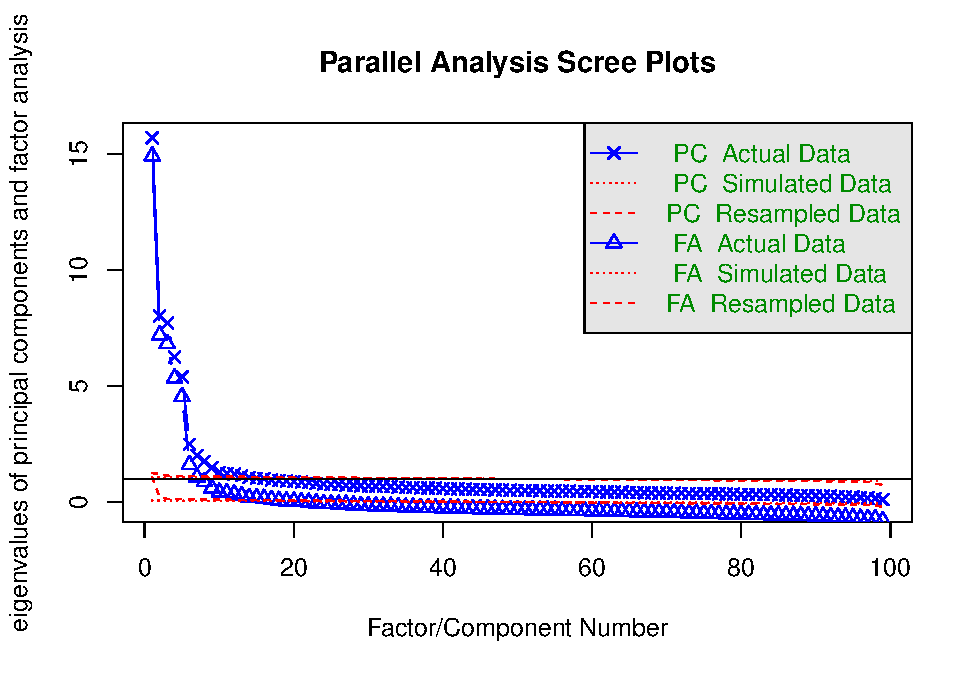
\includegraphics{final_files/figure-latex/\#5 factor structure-1.pdf}

\begin{verbatim}
## Parallel analysis suggests that the number of factors =  20  and the number of components =  14
\end{verbatim}

\begin{Shaded}
\begin{Highlighting}[]
\NormalTok{allFA}\SpecialCharTok{$}\NormalTok{nfact}
\end{Highlighting}
\end{Shaded}

\begin{verbatim}
## [1] 20
\end{verbatim}

\begingroup\fontsize{12}{14}\selectfont

\begin{landscape}
\begin{longtable}[t]{llll}
\caption{\label{tab:KableOuput}Agreeableness Descriptives}\\
\toprule
State & Mean & SD & N\\
\midrule
\endfirsthead
\caption[]{\label{tab:KableOuput}Agreeableness Descriptives \textit{(continued)}}\\
\toprule
State & Mean & SD & N\\
\midrule
\endhead

\endfoot
\bottomrule
\endlastfoot
Alabama & 4.610537 & 0.7744197 & 643\\
Alaska & 4.629332 & 0.7841253 & 555\\
Arizona & 4.596157 & 0.7729134 & 866\\
Arkansas & 4.689144 & 0.7750065 & 577\\
California & 4.663943 & 0.7623445 & 9709\\
\addlinespace
Colorado & 4.631178 & 0.7809921 & 1097\\
Connecticut & 4.634948 & 0.7713774 & 986\\
Delaware & 4.575882 & 0.7144243 & 592\\
Florida & 4.659417 & 0.8070510 & 2936\\
Georgia & 4.688953 & 0.7696673 & 2414\\
\addlinespace
Hawaii & 4.637072 & 0.8284047 & 292\\
Idaho & 4.672925 & 0.7444675 & 340\\
Illinois & 4.729347 & 0.7352130 & 5520\\
Indiana & 4.689507 & 0.7638457 & 1707\\
Iowa & 4.667843 & 0.7655999 & 982\\
\addlinespace
Kansas & 4.678785 & 0.7617303 & 808\\
Kentucky & 4.693537 & 0.7580447 & 820\\
Louisiana & 4.703087 & 0.7277572 & 2030\\
Maine & 4.667634 & 0.7913389 & 356\\
Maryland & 4.707332 & 0.7694775 & 1772\\
\addlinespace
Massachusetts & 4.654854 & 0.7788784 & 1935\\
Michigan & 4.653881 & 0.7815882 & 2549\\
Minnesota & 4.667296 & 0.7423893 & 2104\\
Mississippi & 4.722192 & 0.7991229 & 604\\
Missouri & 4.665174 & 0.7644602 & 1611\\
\addlinespace
Montana & 4.765261 & 0.6641912 & 243\\
Nebraska & 4.641667 & 0.7724856 & 580\\
Nevada & 4.633536 & 0.7698699 & 274\\
New Hampshire & 4.629999 & 0.7428263 & 389\\
New Jersey & 4.669726 & 0.7642500 & 2495\\
\addlinespace
New Mexico & 4.727511 & 0.7475549 & 1199\\
New York & 4.663282 & 0.8054766 & 4942\\
North Carolina & 4.647067 & 0.7780090 & 1454\\
North Dakota & 4.615877 & 0.8189782 & 190\\
Ohio & 4.700273 & 0.7612682 & 3600\\
\addlinespace
Oklahoma & 4.652295 & 0.7867416 & 771\\
Oregon & 4.633837 & 0.7672260 & 1203\\
Pennsylvania & 4.656941 & 0.7579218 & 4758\\
Rhode Island & 4.732280 & 0.7377559 & 422\\
South Carolina & 4.727500 & 0.7352295 & 1010\\
\addlinespace
South Dakota & 4.657946 & 0.8397148 & 172\\
Tennessee & 4.663913 & 0.8098826 & 1133\\
Texas & 4.652647 & 0.7789094 & 4662\\
Utah & 4.665389 & 0.7546368 & 487\\
Vermont & 4.776898 & 0.6847462 & 161\\
\addlinespace
Virginia & 4.722891 & 0.7433986 & 2787\\
Washington & 4.653790 & 0.7633607 & 1742\\
West Virginia & 4.618171 & 0.8055191 & 384\\
Wisconsin & 4.641089 & 0.7689811 & 2377\\
Wyoming & 4.662522 & 0.7447127 & 126\\*
\end{longtable}
\end{landscape}
\endgroup{}

\begingroup\fontsize{12}{14}\selectfont

\begin{landscape}
\begin{longtable}[t]{llll}
\caption{\label{tab:KableOuput}Conscientiousness Descriptives}\\
\toprule
State & Mean & SD & N\\
\midrule
\endfirsthead
\caption[]{\label{tab:KableOuput}Conscientiousness Descriptives \textit{(continued)}}\\
\toprule
State & Mean & SD & N\\
\midrule
\endhead

\endfoot
\bottomrule
\endlastfoot
Alabama & 4.117571 & 0.9667964 & 643\\
Alaska & 4.026173 & 0.8683283 & 555\\
Arizona & 4.098011 & 0.8929967 & 866\\
Arkansas & 4.147743 & 0.9248194 & 577\\
California & 4.095768 & 0.9086644 & 9709\\
\addlinespace
Colorado & 4.124273 & 0.9210228 & 1097\\
Connecticut & 4.120340 & 0.9307941 & 986\\
Delaware & 3.997203 & 0.8632940 & 592\\
Florida & 4.179669 & 0.9343133 & 2936\\
Georgia & 4.129606 & 0.9180854 & 2414\\
\addlinespace
Hawaii & 4.170548 & 0.8806935 & 292\\
Idaho & 4.150588 & 0.8735417 & 340\\
Illinois & 4.162300 & 0.9112091 & 5520\\
Indiana & 4.218357 & 0.9211999 & 1707\\
Iowa & 4.102082 & 0.9230007 & 982\\
\addlinespace
Kansas & 4.108794 & 0.9105627 & 808\\
Kentucky & 4.122991 & 0.9537198 & 820\\
Louisiana & 4.209949 & 0.8955529 & 2030\\
Maine & 4.205641 & 0.9188266 & 356\\
Maryland & 4.128232 & 0.9095782 & 1772\\
\addlinespace
Massachusetts & 4.118530 & 0.9365527 & 1935\\
Michigan & 4.162636 & 0.9299835 & 2549\\
Minnesota & 4.096184 & 0.8982866 & 2104\\
Mississippi & 4.198448 & 0.9059218 & 604\\
Missouri & 4.141600 & 0.9351437 & 1611\\
\addlinespace
Montana & 4.160722 & 0.9577293 & 243\\
Nebraska & 4.156379 & 0.8777856 & 580\\
Nevada & 4.082401 & 0.9495511 & 274\\
New Hampshire & 4.148700 & 0.8946446 & 389\\
New Jersey & 4.148890 & 0.9280449 & 2495\\
\addlinespace
New Mexico & 4.262791 & 0.8985910 & 1199\\
New York & 4.148340 & 0.9339365 & 4942\\
North Carolina & 4.171695 & 0.9481568 & 1454\\
North Dakota & 4.287222 & 0.8787829 & 190\\
Ohio & 4.188897 & 0.9247682 & 3600\\
\addlinespace
Oklahoma & 4.140532 & 0.9454096 & 771\\
Oregon & 4.070511 & 0.9039862 & 1203\\
Pennsylvania & 4.117532 & 0.9191805 & 4758\\
Rhode Island & 4.099572 & 0.9192980 & 422\\
South Carolina & 4.136447 & 0.8851777 & 1010\\
\addlinespace
South Dakota & 4.266537 & 0.8999202 & 172\\
Tennessee & 4.208465 & 0.9470666 & 1133\\
Texas & 4.131076 & 0.9285345 & 4662\\
Utah & 4.102647 & 0.8660975 & 487\\
Vermont & 4.090649 & 0.9496127 & 161\\
\addlinespace
Virginia & 4.141444 & 0.9057514 & 2787\\
Washington & 4.127309 & 0.9222153 & 1742\\
West Virginia & 4.163824 & 0.9387757 & 384\\
Wisconsin & 4.112204 & 0.9268177 & 2377\\
Wyoming & 4.188095 & 0.9480086 & 126\\*
\end{longtable}
\end{landscape}
\endgroup{}

\begingroup\fontsize{12}{14}\selectfont

\begin{landscape}
\begin{longtable}[t]{llll}
\caption{\label{tab:KableOuput}Extraversion Descriptives}\\
\toprule
State & Mean & SD & N\\
\midrule
\endfirsthead
\caption[]{\label{tab:KableOuput}Extraversion Descriptives \textit{(continued)}}\\
\toprule
State & Mean & SD & N\\
\midrule
\endhead

\endfoot
\bottomrule
\endlastfoot
Alabama & 3.744427 & 1.0737088 & 643\\
Alaska & 3.802078 & 1.0298194 & 555\\
Arizona & 3.826485 & 1.0391321 & 866\\
Arkansas & 3.826526 & 1.1045412 & 577\\
California & 3.916162 & 1.0182084 & 9709\\
\addlinespace
Colorado & 3.811444 & 1.0267798 & 1097\\
Connecticut & 3.924073 & 1.0262157 & 986\\
Delaware & 4.029242 & 0.9524545 & 592\\
Florida & 3.888615 & 1.0586144 & 2936\\
Georgia & 3.998944 & 1.0429965 & 2414\\
\addlinespace
Hawaii & 3.835455 & 1.0309916 & 292\\
Idaho & 3.752173 & 1.0263106 & 340\\
Illinois & 4.012087 & 0.9837590 & 5520\\
Indiana & 3.894970 & 1.0577104 & 1707\\
Iowa & 3.907930 & 1.0020006 & 982\\
\addlinespace
Kansas & 3.939745 & 1.0499232 & 808\\
Kentucky & 3.938068 & 1.0360986 & 820\\
Louisiana & 4.010502 & 0.9748960 & 2030\\
Maine & 3.846177 & 1.0208230 & 356\\
Maryland & 3.919828 & 1.0085951 & 1772\\
\addlinespace
Massachusetts & 3.894588 & 1.0272060 & 1935\\
Michigan & 3.896950 & 1.0384003 & 2549\\
Minnesota & 3.941308 & 1.0015734 & 2104\\
Mississippi & 3.920760 & 1.0388218 & 604\\
Missouri & 3.912232 & 0.9806955 & 1611\\
\addlinespace
Montana & 3.847828 & 1.0609354 & 243\\
Nebraska & 3.918702 & 0.9855573 & 580\\
Nevada & 3.816920 & 1.0112589 & 274\\
New Hampshire & 3.862380 & 0.9731819 & 389\\
New Jersey & 3.996112 & 0.9864916 & 2495\\
\addlinespace
New Mexico & 3.898791 & 1.0508917 & 1199\\
New York & 3.933406 & 1.0287508 & 4942\\
North Carolina & 3.802822 & 1.0565457 & 1454\\
North Dakota & 3.803845 & 1.0412612 & 190\\
Ohio & 3.920517 & 1.0329506 & 3600\\
\addlinespace
Oklahoma & 3.804182 & 1.0792374 & 771\\
Oregon & 3.886437 & 1.0061902 & 1203\\
Pennsylvania & 3.958699 & 1.0067223 & 4758\\
Rhode Island & 4.057464 & 0.9397830 & 422\\
South Carolina & 4.043584 & 0.9876283 & 1010\\
\addlinespace
South Dakota & 3.979409 & 1.0081303 & 172\\
Tennessee & 3.847732 & 1.0370815 & 1133\\
Texas & 3.888641 & 1.0537326 & 4662\\
Utah & 3.884845 & 1.0514536 & 487\\
Vermont & 3.917118 & 0.9878257 & 161\\
\addlinespace
Virginia & 3.943700 & 1.0111944 & 2787\\
Washington & 3.809801 & 1.0334914 & 1742\\
West Virginia & 3.779065 & 1.0798027 & 384\\
Wisconsin & 3.920540 & 1.0092239 & 2377\\
Wyoming & 3.821847 & 1.0187586 & 126\\*
\end{longtable}
\end{landscape}
\endgroup{}

\begingroup\fontsize{12}{14}\selectfont

\begin{landscape}
\begin{longtable}[t]{llll}
\caption{\label{tab:KableOuput}Intellect Descriptives}\\
\toprule
State & Mean & SD & N\\
\midrule
\endfirsthead
\caption[]{\label{tab:KableOuput}Intellect Descriptives \textit{(continued)}}\\
\toprule
State & Mean & SD & N\\
\midrule
\endhead

\endfoot
\bottomrule
\endlastfoot
Alabama & 4.637855 & 0.7449558 & 643\\
Alaska & 4.664919 & 0.7668085 & 555\\
Arizona & 4.665397 & 0.7510410 & 866\\
Arkansas & 4.601727 & 0.7666522 & 577\\
California & 4.607159 & 0.7273981 & 9709\\
\addlinespace
Colorado & 4.670469 & 0.7275069 & 1097\\
Connecticut & 4.655686 & 0.7412064 & 986\\
Delaware & 4.386655 & 0.7205952 & 592\\
Florida & 4.657286 & 0.7032552 & 2936\\
Georgia & 4.597719 & 0.7234032 & 2414\\
\addlinespace
Hawaii & 4.533509 & 0.7517126 & 292\\
Idaho & 4.676192 & 0.7004048 & 340\\
Illinois & 4.568339 & 0.7243646 & 5520\\
Indiana & 4.578118 & 0.7459488 & 1707\\
Iowa & 4.533963 & 0.7319487 & 982\\
\addlinespace
Kansas & 4.600704 & 0.7605258 & 808\\
Kentucky & 4.601366 & 0.7377464 & 820\\
Louisiana & 4.421264 & 0.7414032 & 2030\\
Maine & 4.643924 & 0.7361798 & 356\\
Maryland & 4.577738 & 0.7187010 & 1772\\
\addlinespace
Massachusetts & 4.574818 & 0.7139949 & 1935\\
Michigan & 4.656310 & 0.7285229 & 2549\\
Minnesota & 4.531498 & 0.7231444 & 2104\\
Mississippi & 4.559547 & 0.7368477 & 604\\
Missouri & 4.588972 & 0.7330890 & 1611\\
\addlinespace
Montana & 4.708861 & 0.7378293 & 243\\
Nebraska & 4.495270 & 0.7481413 & 580\\
Nevada & 4.651490 & 0.7185546 & 274\\
New Hampshire & 4.630421 & 0.7565377 & 389\\
New Jersey & 4.612689 & 0.7390479 & 2495\\
\addlinespace
New Mexico & 4.579827 & 0.6900077 & 1199\\
New York & 4.649041 & 0.7256438 & 4942\\
North Carolina & 4.569312 & 0.7502207 & 1454\\
North Dakota & 4.570237 & 0.7177782 & 190\\
Ohio & 4.556529 & 0.7364082 & 3600\\
\addlinespace
Oklahoma & 4.605553 & 0.7834762 & 771\\
Oregon & 4.619854 & 0.7436931 & 1203\\
Pennsylvania & 4.512731 & 0.7411906 & 4758\\
Rhode Island & 4.622255 & 0.6808287 & 422\\
South Carolina & 4.485802 & 0.7222830 & 1010\\
\addlinespace
South Dakota & 4.653013 & 0.6828377 & 172\\
Tennessee & 4.590234 & 0.7736854 & 1133\\
Texas & 4.613907 & 0.7484548 & 4662\\
Utah & 4.607547 & 0.7199137 & 487\\
Vermont & 4.735498 & 0.7363306 & 161\\
\addlinespace
Virginia & 4.547663 & 0.7079233 & 2787\\
Washington & 4.684024 & 0.6893191 & 1742\\
West Virginia & 4.582448 & 0.7334187 & 384\\
Wisconsin & 4.504417 & 0.7397412 & 2377\\
Wyoming & 4.631488 & 0.6969593 & 126\\*
\end{longtable}
\end{landscape}
\endgroup{}

\begin{Shaded}
\begin{Highlighting}[]
\FunctionTok{load}\NormalTok{(}\FunctionTok{here}\NormalTok{(}\StringTok{"data"}\NormalTok{, }\StringTok{"statefactor.rda"}\NormalTok{))}
\NormalTok{stateFactordf}
\end{Highlighting}
\end{Shaded}

\begin{verbatim}
##   Alabama Alaska Arizona Arkansas California Colorado Connecticut Delaware
## 1       5      6       5        5          5        5           5        6
##   Florida Georgia Hawaii Idaho Illinois Indiana Iowa Kansas Kentucky Louisiana
## 1       5       5      6     6        5       5    5      5        5         5
##   Maine Maryland Massachusetts Michigan Minnesota Mississippi Missouri Montana
## 1     5        5             5        5         5           6        5       7
##   Nebraska Nevada New.Hampshire New.Jersey New.Mexico New.York North.Carolina
## 1        5      7             6          5          5        5              5
##   North.Dakota Ohio Oklahoma Oregon Pennsylvania Rhode.Island South.Carolina
## 1            7    5        5      5            5            7              5
##   South.Dakota Tennessee Texas Utah Vermont Virginia Washington West.Virginia
## 1            7         5     5    5       8        5          5             6
##   Wisconsin Wyoming
## 1         5       8
\end{verbatim}

\begin{verbatim}
## Downloading ingested version of data with readr::read_tsv. To download the original version and remove this message, set original = TRUE.
\end{verbatim}

\begin{verbatim}
## Rows: 128464 Columns: 390
## -- Column specification --------------------------------------------------------
## Delimiter: "\t"
## chr  (12): gender, relstatus, marstatus, exer, smoke, country, state, ethnic...
## dbl (378): RID, age, height, BMI, weight, q_6, q_22, q_23, q_39, q_40, q_44,...
## 
## i Use `spec()` to retrieve the full column specification for this data.
## i Specify the column types or set `show_col_types = FALSE` to quiet this message.
## Joining, by = "state"
\end{verbatim}

\newpage

\hypertarget{introduction}{%
\section{Introduction}\label{introduction}}

\hypertarget{big-five}{%
\subsection{Big Five}\label{big-five}}

One of the most widely replicated findings within the field of personality psychology is the Big Five structure of personality. With roots in the 1800's, personality psychology sought to determine the best way to represent the large number of personality traits in a concise structure. This research initially involved researchers providing participants with large numbers of trait descriptive adjectives and asking them to rate the extent to which those adjectives characterize themselves or someone they knew. Dimension reduction analyses were then used to create a simpler structure from those responses.

Multiple research groups began converging on the five factor structure as early as the 1960's, with an increasing consensus by the late 1980's. Most of the recent work on the big five has been conducted through a combination of confirmatory factor analysis and theory driven selection of survey items based on previous findings about the structure.

\hypertarget{geographical-personality}{%
\subsection{Geographical Personality}\label{geographical-personality}}

In recent years, there has been increasing focus on regional variation of personality traits within the United States. Work has examined the extent to which regions of the US differ on the Big Five domains and can be said to have distinct and characteristic combinations of trait levels. For example, Rentfrow and colleagues (2013) show that the south and midwest are best characterized as friendly and conventional, whereas the west is relaxed and creative, and the northeast is temperamental and uninhibited.

A limitation of this work is that it examines the extent to which the five factor structure captures each region and what differences in the levels of each factor are due to regional variation. This research utilizes confirmatory factor analyses that assume that the five factor structure is the ideal level of dimensionality to characterize all regions.

\hypertarget{cross-cultural-studies}{%
\subsection{Cross-Cultural Studies}\label{cross-cultural-studies}}

Much of the cross-cultural work on personality structure has found some support for the notion that the five factor structure has applicability in a number of cultures. However, these studies typically are conducted from an etic perspective that translate the items used in western samples.

However, when studies are conducted from an emic perspective -- that is, using trait descriptive adjectives from the language of the culture, rather than translations of items used in the big five framework -- different structures emerge. A varying number of factors have been found to best fit different cultures, ranging from one to seven in many cases.

\hypertarget{geographical-factor-structure-within-us}{%
\subsection{Geographical Factor Structure within US}\label{geographical-factor-structure-within-us}}

Within the US, the regional variation in factor structures has not been an extensively studied topic. Because most research operates within a framework that utilizes confirmatory factor analysis, there is little information on the extent to which regions differ in their factor structure.

In the current study, we use exploratory factor analyses to provide estimates of the optimal factor structures for each of the fifty states.

\hypertarget{brief-methods}{%
\section{Brief Methods}\label{brief-methods}}

\hypertarget{measures}{%
\subsection{Measures}\label{measures}}

The International Personality Item Pool is an open-source repository of personality trait items that have been researched extensively in the big five tradition. The current study uses ninety nine of one hundred items from the IPIP-100. Participants rated themselves on a number of personality traits from 1- not at all like me to 6- very much like me.

\hypertarget{data-collection}{%
\subsection{Data Collection}\label{data-collection}}

Data were obtained from the Harvard \href{https://dataverse.harvard.edu/dataverse/SAPA-Project}{Dataverse}. Data were initially collected using the Synthetic Aperture for Personality Assessment (Revelle et al., 2016; Condon and Revelle, 2014; Wilt et al., 2011; @DVN/2IBBMG\_2021) which utilizes a massively missing completely at random design, wherein each participant only provides responses to a fraction of items.

\hypertarget{analyses}{%
\section{Analyses}\label{analyses}}

First, we provide descriptive norms for the entire US sample, and then by state.

Next, we use parallel analysis to determine the optimal number of factors in the whole sample. Our hypothesis is that five factors will provide an optimal fit.

The main analyses are fifty parallel analyses, one for every state, that estimates the optimal number of personality dimensions for each state. We hypothesize that there will be variation in the number of ideal dimensions across states.

\newpage

\hypertarget{results}{%
\section{Results}\label{results}}

The parallel factor analyses indicate that the modal number of factors is 5, as is found in 36 of the 50 states, with 7, 6, and 1 states respectively being better represented by 6, 7, and 8 factors.

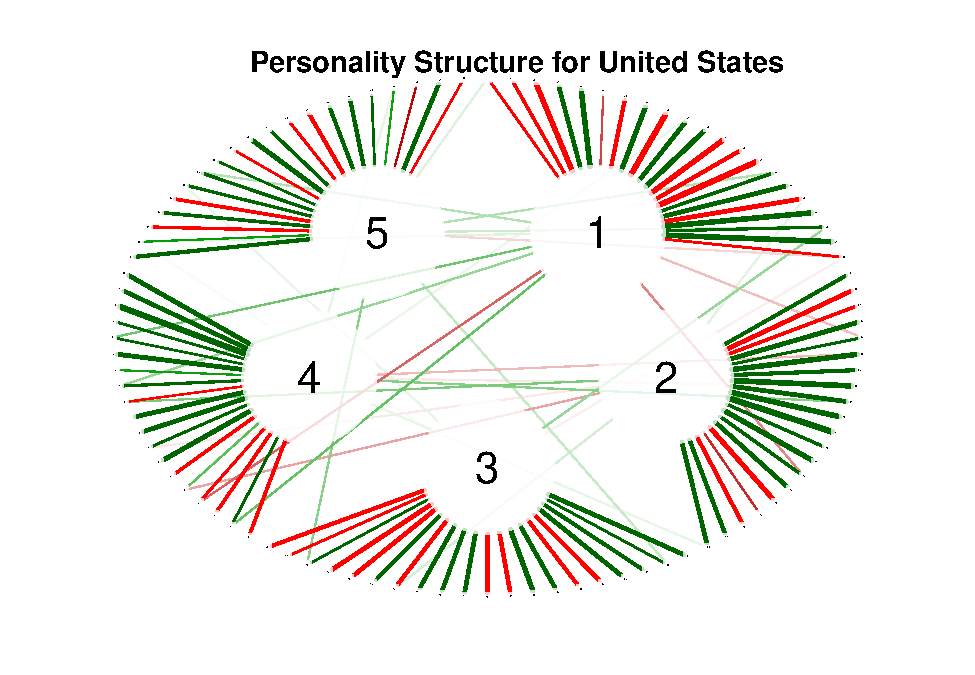
\includegraphics{final_files/figure-latex/unnamed-chunk-3-1.pdf} 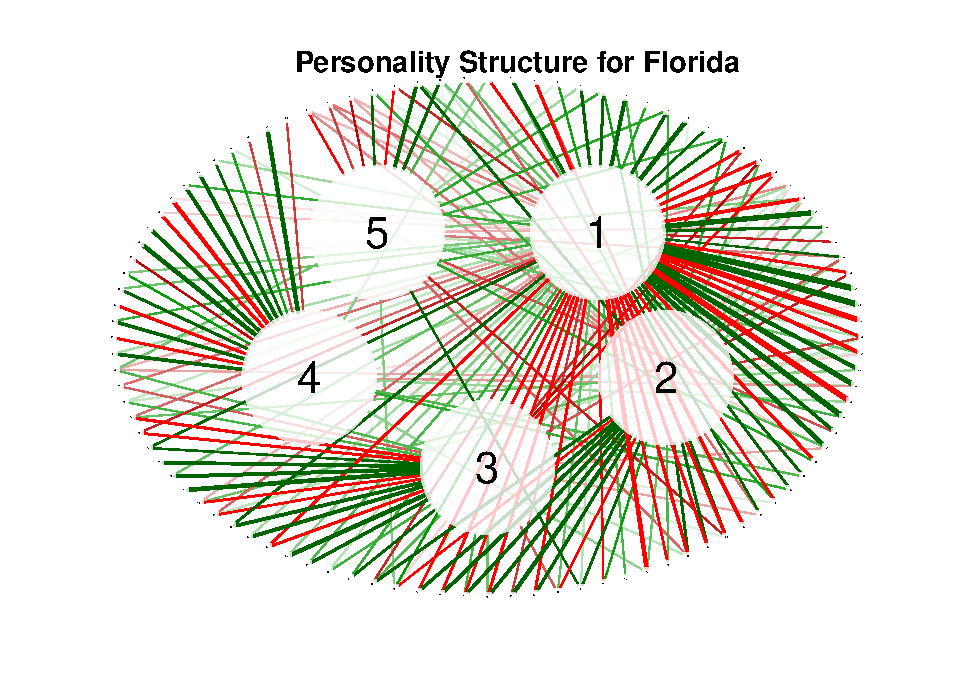
\includegraphics{final_files/figure-latex/unnamed-chunk-3-2.pdf} 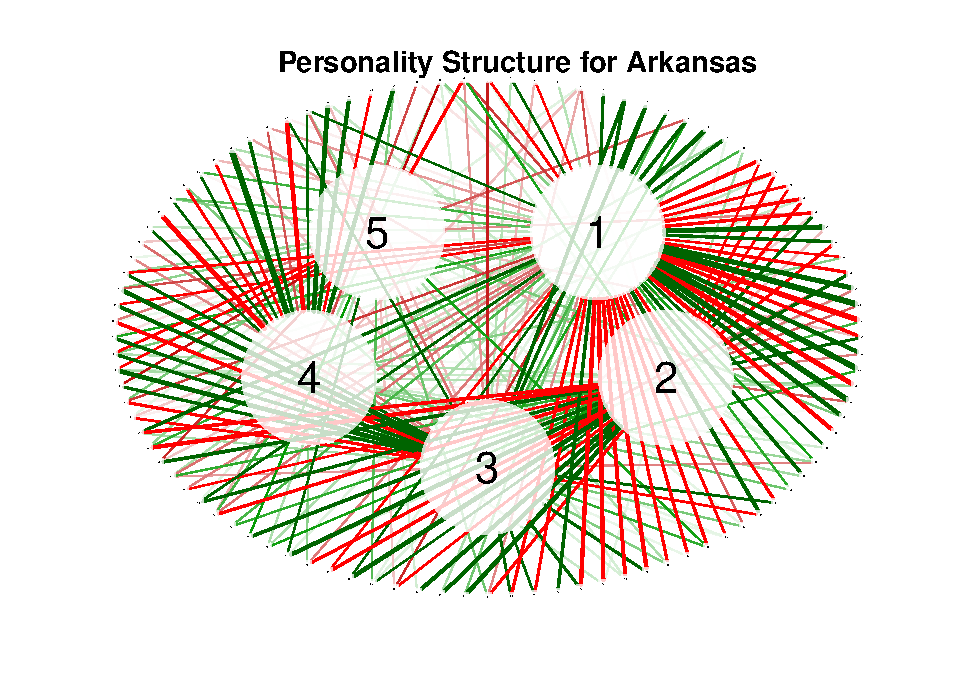
\includegraphics{final_files/figure-latex/unnamed-chunk-3-3.pdf} 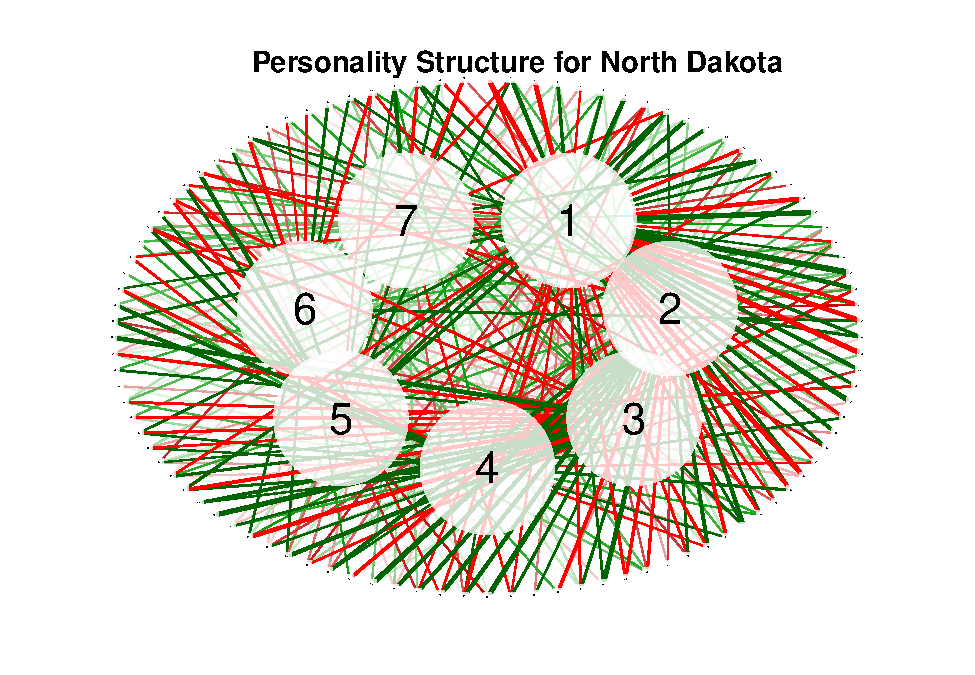
\includegraphics{final_files/figure-latex/unnamed-chunk-3-4.pdf}

\hypertarget{ek-peer-review}{%
\subsubsection{EK Peer Review:}\label{ek-peer-review}}

\hypertarget{areas-of-strength}{%
\section{Areas of strength:}\label{areas-of-strength}}

\begin{enumerate}
\def\labelenumi{\arabic{enumi}.}
\tightlist
\item
  Awesome use of branches/git features in general! Made it clear to see who was working on what sections, and how the project was arranged.
\item
  Code is arranged easily to read, nice use of sections and not doing more than 1\textasciitilde2 things per line of code.
\item
  Great reproducibility with having data loading working on first try for me, and doesn't require any extra files/folders outside of the ``scripts'' folder- might be beneficial to cache the data however?
\end{enumerate}

What I learned: Familiarity with the IPIP dataset! I'd really like tos ee some visualizations on how these factors vary across the different states, maybe using a geographic visualization?

\hypertarget{ek-suggestions}{%
\section{EK Suggestions:}\label{ek-suggestions}}

\begin{itemize}
\tightlist
\item
  Code cleanup: moved library declarations to teh beginning of the script, and added the ``needs'' package'' to simplify package loading
\end{itemize}

\end{document}
